% Chapter Template

\chapter{Experimental Setup} % Main chapter title

\label{Chapter3} % Change X to a consecutive number; for referencing this chapter elsewhere, use \ref{ChapterX}

\lhead{Chapter 3. \emph{Experimental Setup}} % Change X to a consecutive number; this is for the header on each page - perhaps a shortened title

%----------------------------------------------------------------------------------------
%	SECTION 1
%----------------------------------------------------------------------------------------

\section{Expansion Tube}

The expansion tube is an impulse flow device similar to a shock tube. With an expansion tube, a high pressure gas is used to accelerate a volume of lower pressure gas to certain conditions required for supersonic testing. For the case of supersonic cavities, these conditions need to be similar to those found in the combustor of a scramjet engine. With the expansion tube at Lafayette College, Mach numbers between 2 and 4 have been attained. 

%-----------------------------------
%	SUBSECTION 1
%-----------------------------------
\subsection{Sections}

The expansion tube consists of four sections, which are highlighted in Figure \ref{fig:tubelabeled}. The four sections are: the driver, the double diaphragm, the driven, and the expansion, as listed from upstream to downstream. Initial conditions of the tube set by the operator determine test conditions within test section. These initial conditions include pressure ratios between the sections as well as the gases used in the sections. Each section is divided by plastic diaphragms at the start of each tests. These diaphragms allow the sections to be filled to the different pressures with the different gases required for testing.

The driver section is contained at a high pressure at the start of a test. This section is rated to be filled up to 800 psi. Non-combusting tests performed were run with a driver pressure of 225 psi. With higher pressures, faster test velocities of the test gas can be achieved. 

The double diaphragm serves as a starting mechanism for the experiments. It is filled to an intermediate pressure about half the driver pressure. This section is a very small volume, which when vented, rapidly creates a large pressure drop across the most upstream diaphragm, causing it to break. The breaking of the diaphragm begins a chain reaction, starting the test. 

Once the test begins, the test gas, which is contained in the driven section at a sub-atmospheric pressure, is accelerated by the driver gas. The test gas travels down the tube, compressed and shock heated until it breaks through the last diaphragm between the driven and expansion sections. This last section differentiates an expansion tube from a shock tube. With the addition of the last diaphragm, the expansion section can be kept at an even lower pressure than the driven section. When the diaphragm between these sections break, the test gas experiences  expansion and unsteady acceleration, allowing faster freestream velocities and higher Mach numbers in the test section. 

%-----------------------------------
%	SUBSECTION 2
%-----------------------------------

\subsection{Diaphragms}
To separate the four sections, plastic diaphragms were placed at the boundary between these sections. These diaphragms were used to keep a pressure differential between the driver, double diaphragm, and driven sections. The pressure differential between these sections was a maximum of 120 psi for non-combusting tests. Another diaphragm was used to separate the test gas in the driver and the expansion gas in the expansion section. Depending on the test conditions, this diaphragm was required to withstand a maximum pressure differential of 1 psi. 

Different thickness diaphragms were required, depending on the pressure differential between the sections. All diaphragms used for the driver and double diaphragm sections were cut from polycarbonate sheet. In order to determine the required diaphragm thickness, calculations were performed, utilizing known material properties and spherical pressure vessel relationships. Since the diaphragm is expected to expand to a near half sphere before breaking, a thin wall spherical pressure vessel relationship was used to determine the maximum pressure the plastic could withstand. This relationship, shown in Equation \ref{eq:spherePV}, was utilized to determine a range of thicknesses of the polycarbonate sheets to be used for different pressure conditions. 

\begin{equation}
\sigma_{uts} = \frac{P~r}{2t}
\label{eq:spherePV}
\end{equation}

After initial testing of these diaphragms, it was determined this relationship provided an overestimation of about 185\% for the breaking pressure of a specific thickness of diaphragm. Since the polycarbonate sheets come in certain stock thicknesses, several thicknesses were purchased and testing was performed to determine the breaking pressure of each diaphragm. For this testing, a 1/4" polycarbonate sheet was placed at the upstream end of the double diaphragm and the thinner test sample was placed at the downstream end of the double diaphragm. The double diaphragm was then filled slowly. When the downstream diaphragm broke, the highest pressure reached was recorded. This procedure was repeated for other thicknesses of diaphragms. The results from these burst tests is shown in Table \ref{Table:Burst}. A majority of the non-combusting tests run were at a driver pressure of 225 psi, so 0.045" diaphragms were selected, as they have a higher burst pressure than the pressure differential between the driven and the double diaphragm, but not higher than the differential between the driver and the driven sections. These diaphragms reliably broke for each test.

\begin{table}
\centering
\begin{tabular}{|c|c|c|}
\hline
\hline
Thickness (inches) & Trial 1 Burst Pressure (psi) & Trial 2 Burst Pressure (psi)\\ 
\hline \hline
0.010 & 32 & n/a \\

0.015 & 60 & n/a \\

0.020 & 93 & 92 \\

0.030 & 123 & 125 \\

0.045 & 153 & 163 \\

1/16 & 233 & 274 \\

3/32 & 341 & n/a \\

\hline \hline

\end{tabular}
\caption[Diaphragm Burst Pressures]{Diaphragm burst pressures at various thicknesses of polycarbonate sheets.}
\label{Table:Burst}
\end{table}

Occasionally, after a test was run, it was noticed that the pieces of the diaphragm completely broke off, sending these pieces down the tube. Having these large pieces of diaphragm sent down the tube is unwanted. These large pieces can cause serious damage to the model in the test section, as well as damage to other parts of the tube. During one test, a large piece of diaphragm struck the nose of the blunted cylinder model, causing severe damage to the pressure transducer located at the nose. It was also observed that pieces of diaphragm nicked the observation windows on the test section. These damages needed to be avoided, so one proposed solution to this problem was to score the diaphragms. A short, shallow incision on the outside of the plastic in an "X" pattern would create failure modes which the diaphragm should break along. These failure modes cause the diaphragm to petal, ideally opening as wide as the tube, with the entire diaphragm intact. 

Burst tests were performed on several scored diaphragms of 0.045" thickness.  This scoring was performed by hand with a knife, applying light pressure. The resulting score appeared as deep scratches in an "X" pattern. The results of the tests showed no significant decrease in burst pressure. In fact, all of the tests showed a higher burst pressure for the scored diaphragms than for the not scored ones. This could be due to the scoring allowing the plastic to deform further before bursting. It could also be due to the plastic being from a different batch sheet than the plastic used for earlier burst tests. Regardless of the reason, the results showed that the scored diaphragms could still be used. It was also found that good petalling of the diaphragm occurred, with minimal, if any, loss of diaphragm pieces down the tube. Because of these results, scoring of the diaphragms has become a regular step in the setup of the tube for each test.  




%----------------------------------------------------------------------------------------
%	SECTION 2
%----------------------------------------------------------------------------------------

\section{Models}

For testing, a cavity model was designed and manufactured. The designed cavity, as shown in Figure \ref{fig:cavModel}, was designed to be mounted with the current mounting system in the test section. This mounting system consists of a rectangular upright with thru holes for shoulder bolts. The three holes seen in Figure \ref{fig:cavModel} are in line with the existing holes in the mounting system. This allows one to swap out models in the test section quickly in between tests. 


%-----------------------------------
%	SUBSECTION 1
%-----------------------------------
\subsection{Design Choices}

While designing the cavity, several choices had to be made about the geometry of the model as well as the features of the cavity. Brass was chosen as the material due to its relatively low cost as well as its ability to be easily machined. Brass also holds up well to the conditions experienced in the test section during testing. 

The overall size of the brass was chosen based on the size of the core flow, the flow volume where the desired freestream conditions exist, exiting the tube into the test section as well as the requirement to be affixed to the existing mounting system. The size of the core flow coming out of the tube begins about the diameter of the tube itself. However, it grows smaller as the length from the tube exit increases. It is important that the area of interest (the cavity) is contained entirely within this core flow. Knowing the cavity would sit a few inches from exit of the tube, a width of 2.5 inches was chosen for the brass. This would ensure that the core flow, at the time it interacts with the cavity, would entirely encapsulate the cavity. A total height of 1 inch was chosen because it allowed the rectangular hole for the mounting system to be machined to the correct depth that aligned the thru holes for the shoulder bolts. It was designed that after the rectangular hole was made in the brass, a thickness of 1/4 inch was left. This was chosen because the cavity exists relatively close to the mounting system and at least 1/8 inch of material needed to be left between the top of the mounting system and the bottom of the cavity to ensure the part could be machined without any issues. 

The cavity itself was placed \textbf{THIS FAR AWAY FROM THE FRONT} in order to develop the flow over the flat plate. Flow conditions experienced by the cavity should match closely to flow conditions experienced in scramjet engines, including boundary layer conditions. The thickness of the boundary layer was estimated to be on the order of \textbf{Blank} for the length chosen. This estimation was made using the relationship shown in Equation \ref{eq:BL}, where Re is shown by the relationship in Equation \ref{eq:Re} and x is the distance to the front of the cavity from the leading edge of the model. For consistency with other researchers and their boundary layer thickness, as length of \textbf{THIS LENGTH} was chosen.

\begin{equation}
\delta = \frac{0.37x}{(Re_x)^{1/5}}
\label{eq:BL}
\end{equation}

\begin{equation}
Re_x = \frac{\rho U_\infty x}{\mu}
\label{eq:Re}
\end{equation}

At the upstream end of the cavity model, there exists a wedge. Flow over a flat plate leading up to the cavity was desired. The wedge was designed in order to redirect any shock waves away from the cavity. These shock waves have the ability to adversely affect test results if they interact with the cavity. Calculating shock wave angles for several wedge angles and calculating where the shocks would reflect off the walls of the test section, a wedge angle of 20$^\circ$ was chosen. This angle created a shock of about 46$^\circ$ for a freestream mach number M$_\infty$ of 2.5 and a specific heat ratio, $\gamma$ of 1.4, which are conditions similar to the ones that will be run for the cavities. When reflected through the shear layers surrounding the expansion tube core flow, the oblique shock produced would not reflect into the cavity.

The stability of the model was also an important design consideration. With the flow conditions experienced in the test section, a stagnation pressure of nearly 1,000 psi could be experienced by the model. With the model's front wedge shape, a net force in the vertical direction of nearly 3,300 lbs., coupled with a relatively large moment arm has the potential to result in some movement from the cavity. Initial calculations of bending resulted in a maximum deflection of around 0.05 inches. These calculations assumed the model to have a uniform rectangular cross section and all the force was in the center of the wedge. To ensure the bending was as minimal as possible, a triangular brace was manufactured to secure the base of the cavity to the test model stand. This reduced the effective moment arm to provide structural support and stability to the model. This triangular support is pictured in the test section assembly in Figure \ref{fig:cavTestSection}.


%-----------------------------------
%	SUBSECTION 2
%-----------------------------------
\subsection{Modular Design}

Because the acoustic properties are the main focus of this thesis, it was important to design a model in which these acoustic properties could change. Frequency is one main acoustic property that was chosen to be varied with these cavities. Using Heller and Delfs relationship, Equation \ref{eq:freq}, varying the length of the cavity would lead to different cavity frequencies \cite{heller1996letter}. However, the L/D is also an important parameter in the flame-holding characteristics of these cavities. This ratio determines the recirculation properties as well as residence time within the cavity. A modular design was then chosen so that a range of L/D ratios could be tested. For good flame-holding characteristics, a L/D between 4 and 10 has been shown to provide those characteristics \cite{ben2001cavity}. For the design, having a constant depth would result in a change in length of the cavity with a change in L/D ratio. Thus, as the L/D ratio changes, so do the flame holding properties as well as the dominant frequencies within these cavities. 

For the modular design, a 1/8-inch deep, 1 5/8-inch long cavity was created, as shown in Figure \ref{fig:cavModel}. Along with the large cavity, different sized inserts were manufactured. The length of the cavity was chosen so that these inserts could be attached, decreasing the overall length of the cavity, and achieving the desired L/D. Six inserts were manufactured to create L/Ds of 5, 7, and 9, each with two varients of a downstream wall. These inserts are shown relative to the base cavity in Figure \ref{fig:cavInserts}. At each L/D, there was one insert with a flat wall and one insert manufactured with a 30$^\circ$ incline. This angled incline, as shown by Ben-Yakar \cite{ben2001cavity}, has the ability to suppress the acoustic waves while still retaining flame holding characteristics. The angled wall does not allow the pressure waves to propagate within the cavity space. This allowed for the comparison of flame-holding abilities of the cavity with and without strong acoustic waves present at each L/D. This modular design gave a relatively wide spectrum of cavity conditions to test with a relatively easy means of changing these conditions for each test. 

%-----------------------------------
%	SUBSECTION 3
%-----------------------------------
\subsection{Implementation}

For each test, it was determined which L/D needed to be tested. After this choice was made, the corresponding insert was installed and the test section mount was prepared for the cavity model to be placed in it. Depending on which model was mounted in the test section before the cavity test, the mounting stand may have needed to be adjusted.  Since the area of interest is the cavity, it was placed at the center of the viewing window for the schlieren to focus directly on it. Once the test mount was correctly positioned, the cavity model was attached to it with three shoulder bolts. The triangle support was then attached between the model and test stand, providing extra stability when the test runs. Once the model is mounted, switching between L/D inserts is as easy as removing the test section door and three screws holding the cavity insert to the model. A photo of the cavity installed in the test section is shown in Figure \ref{fig:cavTestSection}.


%----------------------------------------------------------------------------------------
%	SECTION 3
%----------------------------------------------------------------------------------------

\section{High Speed Pressure Transducers}

Placed along the tube at various locations are piezoelectric pressure transducers. These pressure transducers provide both analog and digital data for each test run. The analog data allows for the observation of shock strength and the digital data allows for the calculation of shock velocity. When the shock passes by one of these sensors, it registers as a very sharp increase in pressure. Knowing the time at which these shocks arrive at the various transducer locations, along with the location of the transducers relative to each other allows for the shock speed calculation. 

Ideally, calculating the time step between the arrival of each shock could be done by observing the time between the sharp spike in the analog pressure signal. However, to achieve a more accurate calculation of the time, a digital National Instruments card with a maximum sampling frequency of 20 MHz was used. The faster sampling frequency allows the small time step to be calculated far more accurately than the analog National Instruments card used for the analog pressure signals. 

In order to produce the digital signal required for the LabVIEW timer counter program to calculate the time between signals, a simple analog to digital circuit was designed. The design of the circuit was based off of previous work done by Helen Hutches \cite{Hutchens2015}. This circuit, as shown in Figure \ref{fig:timercircuit}, produces a 5V signal when an analog voltage is higher than a certain threshold. This threshold reference voltage is determined by three potentiometers connected to the circuit. The three potentiometers allow three different reference voltages to be set for up to six pressure transducer signals. When the analog voltage is lower than this reference voltage, the output of the circuit is 0V. This allows the digital data acquisition card to read either a HIGH (5V) signal or a LOW (0V) signal and interpret that as a digital signal. 

This digital signal is also used to trigger the camera to record. The LabVIEW program, once getting a signal from a specified pressure transducer will generate a 5V TTL pulse. 

%-------------------------------------------------------------
%	 SUBSECTION 1
%-----------------------------------------------------------

\subsection{Circuit}
The circuit operates using three op-amps and one pull up resistor. The op-amps, as shown in the center of Figure \ref{fig:timercircuit}, read the signal from the potentiometers. The voltage level, between 0 and 5 volts, from the potentiometer is set by the user. The op-amp compares this voltage to the voltage signal received through the BNC connectors. These BNC connectors are the analog voltage from the pressure transducers along the tube. If the voltage coming from the pressure transducers is below the voltage set by the user, the output of the circuit is 0V or a LOW digital signal. If the voltage is above this set voltage, the output of the circuit is 5V or a HIGH digital signal. 

The purpose of this circuit is to convert the analog signal sent by the pressure transducers into a digital pulse that can be read by the digital card. The potentiometers are put in place so the digital pulse is only sent when the shock wave passes by the transducer, rather than noise actuating the digital signal to be sent. Reliable results have been achieved with this circuit, but there are some cases in which this system has failed, but in the next section, it will be explained how to fix some of the more common problems and check for specific errors.


%----------------------------------------------------------
%	 SUBSECTION 2
%---------------------------------------------------------

\subsection{Implementation and Troubleshooting}

When using the timer counter box, make sure the box is plugged into the power supply. Once the box has power, turn on the power supply associated with the inverting circuit. Once these are powered, the blue amplifier boxes should be turned on to supply power to the transducers. Set the appropriate gains on these boxes. The appropriate gains are based on what magnitude signal is desired. The LabVIEW program will only read signals between 0 and 5V. The pressure transducers output 0-5V for a pressure range of 0 to 100 psi. However, the pressure these transducers will be exposed to are only between 10 and 20 psi, resulting in a 0.5 to 1V signal. Setting the gain to 5 allows that signal to be amplified to to between 2.5 and 5V. Having a larger signal allows for the comparator circuit to operate more easily. One can set the comparator nominal voltage with confidence, as the larger signal allows for a larger margin of error on the set comparator voltage. This gives more confidence that the signal coming into the comparator circuit will be large enough to trigger a digital signal. 

Once the physical systems are powered and ready, run the two LabVIEW programs for the capturing of the digital signals as well as the analog signals. The analog program filename is ''BasicHighSpeedOscillosope-fixed.vi'' and the digital program filename is ''CountersWorking.vi'' For the analog signal, an input is required for sampling rate and time to take data. The typical sampling rate and time for tests is 1MHz and 10,000 $\mu$s. The digital program asks for a user input of ''milliseconds to wait.'' This is the amount of time the program should wait until sending the 5V TTL pulse to the camera. Typically, this value is set to 0. 

One common problem with this circuit is that no digital signal is sent from the circuit itself. To check for this, use a function generator and an oscilloscope. Hook up the oscilloscope to one of the digital out wires of the box as well as the output of the function generator. Table \ref{Table:pins} shows the number of the digital out wire to its corresponding number. Attach the function generator to the corresponding BNC connector. A T-connector is needed to split the output signal from the function generator. Send a 5V amplitude sine wave from the function generator. The corresponding signal from the box should be a square wave. If there is no square wave present, check that the potentiometer is not too high or too low. The square wave should get wider or narrower depending on the position of the potentiometer. If there is still no signal coming from the box, there may be a burnt out op-amp. If, however, there is no signal coming from any of the outputs, it is unlikely all of the op-amps burned out. In this case, there may be a wiring issue. For this, check continuity between the signal coming in and the signal coming out to make sure voltages at each connection are what they are supposed to be. Some alteration of the circuit may be required in this case. However, that is unlikely, and the problem is likely to be that the potentiometer level was set too high.




%---------------------------------------------------------
%    SECTION 4
%-----------------------------------------------------------------------------------

\section{Infrared Sensor}

Test time is important for the correlation of schlieren image data. Because the two systems are initiated simultaneously, the IR data corresponds easily to the image data. Knowing when the test gas reaches the model and for how long the test gas is flowing over the model allows for the extraction of frames that equate to just the test time. Although it is possible by inspection to see when the test gas arrives at the model, it is not always obvious or as accurate. The arrival of the test gas produces shock waves at a different angle than the helium behind the incident shock wave, but this change in angle might not be very large, depending on the change in velocity. However, with the IR data, it can be closely estimated when the test gas should reach the model and for how long the model experiences the test gas. 

Test time can be estimated using an X-T diagram. A sample X-T diagram is shown in Figure \ref{fig:XT}. This diagram is generated using compressible flow equations under an inviscid assumption. The lines represent important flow characteristics, including shock wave or expansion fan locations. The x-axis represents the spatial location along the tube, while the y-axis represents time. The time between the second and third line at the test section location represents the time which the test gas passes by the test section at the proper conditions. This ideal test time can be used to estimate the experimental test time, but a more accurate measurement of test time using the IR sensor is needed for proper image correlation and analysis.

The sensor used with the expansion tube at Lafayette is a Judson J10D series Indium Antemonide (InSb) sensor. These detectors have photovoltaic sensors that produce a current when exposed to infrared radiation. The sensor has the ability to be utilized for both absorption as well as emission sensing techniques. These techniques are explained in detail in a subsequent subsection.

%------------------------
%    SUBSECTION 1
%------------------------

\subsection{Design of System}
The alignment and placement of the various components is important for the proper collection of the IR light from the tube. The setup, as depicted in the diagram in Figure \ref{fig:IRschematic}, includes a slit, a concave mirror, and a flat mirror. The slits affect the spacial resolution of the incoming signal. If the slits are too wide, the sensor captures some of the scattered light, which shows up as a gradual increase in signal. If the slits are too narrow, not enough light can be captured by the sensor to show a good signal. The slit width is still being fine-tuned for the system in place, but the typical width for the slits is between 1 and 3 mm \cite{flower1976experimental}. 

The sensor itself has a circular pickup area of about 2mm in diameter. Because of this, the IR light from the tube needs to be focused. Once the light passes through the slits, it reflects off of a concave mirror. This concave mirror, with a focal length of \textbf{insert focal length}, focuses the light to a small point, just about the size of the sensor. The flat mirror is used to collapse the system so it can fit in a relatively small area. The entire system is contained in a box, as shown in Figure \ref{fig:IRlabel}. Both mirrors are gold coated, as gold is very efficient at reflecting IR light. Since most of the testing is done during the day, a box was constructed to block out any ambient light from the room. The system is attached to the support structure of the tube by a 1/2" aluminum plate cantilever. Some bending, less than 1/16",  is present at the end of the beam where the setup is supported, but it is not enough to affect the collection by the IR system. 

%------------------------
%	 SUBSECTION 2
%------------------------

\subsection{Set Up}


To achieve the sensitivity required for the sensor, the operating temperature of the IR detector is about 77K, and the detector must be cooled with liquid nitrogen. Using the funnel to avoid spillage of the liquid nitrogen onto the cable connections or viewing window of the sensor, a few hundred milliliters were poured into the hole at the top of the sensor. When the sensor reaches the correct temperature, an eruption of cool gas occurs. It is important to wait until this eruption completes because the buildup of gas can cause the cap to blow off. Once the eruption subsides, the cap can be replaced to the top of the sensor and power can be supplied to the amplifier. 

After power is supplied to the sensor through the amplifier, it is important to check that the system is aligned. Since the setup is attached to the support structure and not the tube itself, the recoil of the tube or the moving of the tube to replace diaphragms can alter the alignment of the window to the focusing mirror. To re-align the system, a stainless steel LED tube was constructed. This tube fits within the porthole on the back side of the tube, aligned with the port for the IR sensor. With the LED on and lined up with the inside wall of the far side of the tube, check the light source path. Be sure that the thin slit of red light hits the small sensor area. Adjust the flat mirror as needed to align the slit of red light with the IR sensor pickup area. Once the system is aligned, remove the LED tube and replace the plug in that port. The system at this point is aligned and ready for a test.  

%------------------------
%     SUBSECTION 3
%------------------------

\subsection{Absorption}

One method of data capturing that can be used is infrared absorption. The absorption method is based on the principle that different gases absorb radiation at different amounts. For absorption tests, an infrared light is placed behind a sapphire window on the other side of the tube. This IR light source provides the sensor with a baseline IR emission reading. As different gases pass by the sensor, they absorb some of the IR light, resulting in a different level of IR signal at the sensor. Measuring the time at the absorption level that corresponds to the test gas corresponds to the test time within the test section. Although the sensor is capable of reading the IR signal with this method, the emission method has provided more reliable measurements of test time. The emission method only allows for signal to come to the sensor when the hot test gas is passing by, whereas the absorption method also shows when the other gases pass by the sensor. A typical voltage trace of the absorption method is shown in Figure \ref{fig:IRabsorption}. It is clear that there is much uncertainty of which test gases are passing by the IR sensor during this pressure trace. There are no sharp spikes in signal, but rather, the signal exhibits low sloped voltage changes. Also, at the end of the test, the IR signal should return to its baseline. However, the signal continues to rise, and even experiences a hump near the end of the test. This uncertainty in the voltage trace made it difficult to experimentally measure test times. Because of this, the emission method has been used primarily in the non-combusting tests and will continue to be used in the combustion tests. Further testing and tuning of the system would be required to capture more meaningful information with this absorption method. 


%------------------------
%     SUBSECTION 4
%------------------------

\subsection{Emission}

As gases are heated, they emit IR radiation at different wavelengths. Using a filter, other wavelengths that are not these specific wavelengths, will not pass to the detector. For the non-reacting flows, a 5\% CO$_2$ in nitrogen mixture emits IR within a 180nm bandwidth centered at 4.248$\mu$m. Placing the filter in front of the sensor allows the sensor to detect when, and for how long, the test gas, CO$_2$ passes by the sensor. Knowing how long the gas passes by the sensor allows for a direct measurement of test time in the test section. Due to the sensor's close proximity to the test section, the test time extracted from the IR data is very close to the test time for the models in the test section. An example of the voltage trace produced by the sensor using the emission method is shown in Figure \ref{fig:IRemission}. 



It is also noted that the voltage trace does not exhibit sharp spikes in signal. This is due to the size of the slit width, which was too open for this test. This slit width allowed forward-scattered light to be picked up by the sensor. It was assumed that the true start of the signal is halfway up the slope. However, it is important to continue fine-tuning the system and the slit width in order to eliminate this uncertainty.

%-------------------------
%      SUBSECTION 5
%-------------------------
\subsection{Premature Ignition}

The IR sensor will also be used to determine if pre-combustion occurred during a test. It is expected that if the reaction combusts upstream of the test section, it will result in a very large spike in IR signal. This will indicate that combustion did not originate at the cavity, but rather upstream of the cavity. Since the combustion tests are being used to test the flame-holding characteristics of the cavity, it is imperative that ignition originates at the cavity. 


%---------------------------------------------------------
%    SECTION 5
%-----------------------------------------------------------------------------------

\section{Schlieren Imaging}

The images captured for the tests were done so using a high speed camera with a z-type schlieren system. A diagram of the schlieren system at Lafayette can be seen in Figure \ref{fig:schlieren}. The camera used for image capturing is a Phantom Miro m310 camera, capable of taking images up to 250,000 fps. However, as the recording frame rate increases, the resolution of each image decreases. For testing, a nominal frame rate of 77,000 Hz was used, as this provided a sufficient frame rate without sacrificing too much resolution. The resolution at which the images were taken at in this study is \textbf{Frame Rate Here}. A sufficient frame rate in this context is one in which one test is captured within 500-1,000 frames. Also, to observe the frequencies within the cavity, the frame rate must be several times higher than the expected frequency of the acoustic waves. With L/D of 5, 7, and 9 having expected frequencies of 30 kHz, 21.4 kHz, and 16.7 kHz, respectively, a frame rate of 77 kHz would provide between 3 and 5 frames to observe the propagation of the waves.

The schlieren effect operates on the principle that light refracts in air due to changes in density. This can be observed firsthand on a hot day. The rippling effect one can see above a road on a hot day is the light refracting due to the different densities of the air, caused by differences in local air temperature. Schlieren imaging takes advantage of this principle by placing a knife edge at the focal point of the system. As light is refracted due to a change in density, this light gets blocked out by the knife edge, showing up as a dark spot in the captured image. Light that is not refracted continues through to the camera unblocked. 

This type of imaging is important to see the various shock waves produced during testing. Since shock waves produce very sharp density gradients, a system that is capable of capturing these density gradients at high speeds is very useful. Typical test time of the non-reacting tests, the time in which the model experienced the test gas,  was on the order of about 300 microseconds. With this camera, nearly 23 images were captured for the test time.  With this many frames, it was possible to time correlate the images as well as extract dominant frequencies within the cavities.

Further information about the system, including more detail on how the system works and how to calibrate and align the system at Lafayette can be found in Ray Sanzi's honors thesis \cite{Sanzi2016}.



%-------------------------------------------------------------------
%    FIGURES
%------------------------------------------------------------
\newpage

\begin{sidewaysfigure}
\centering
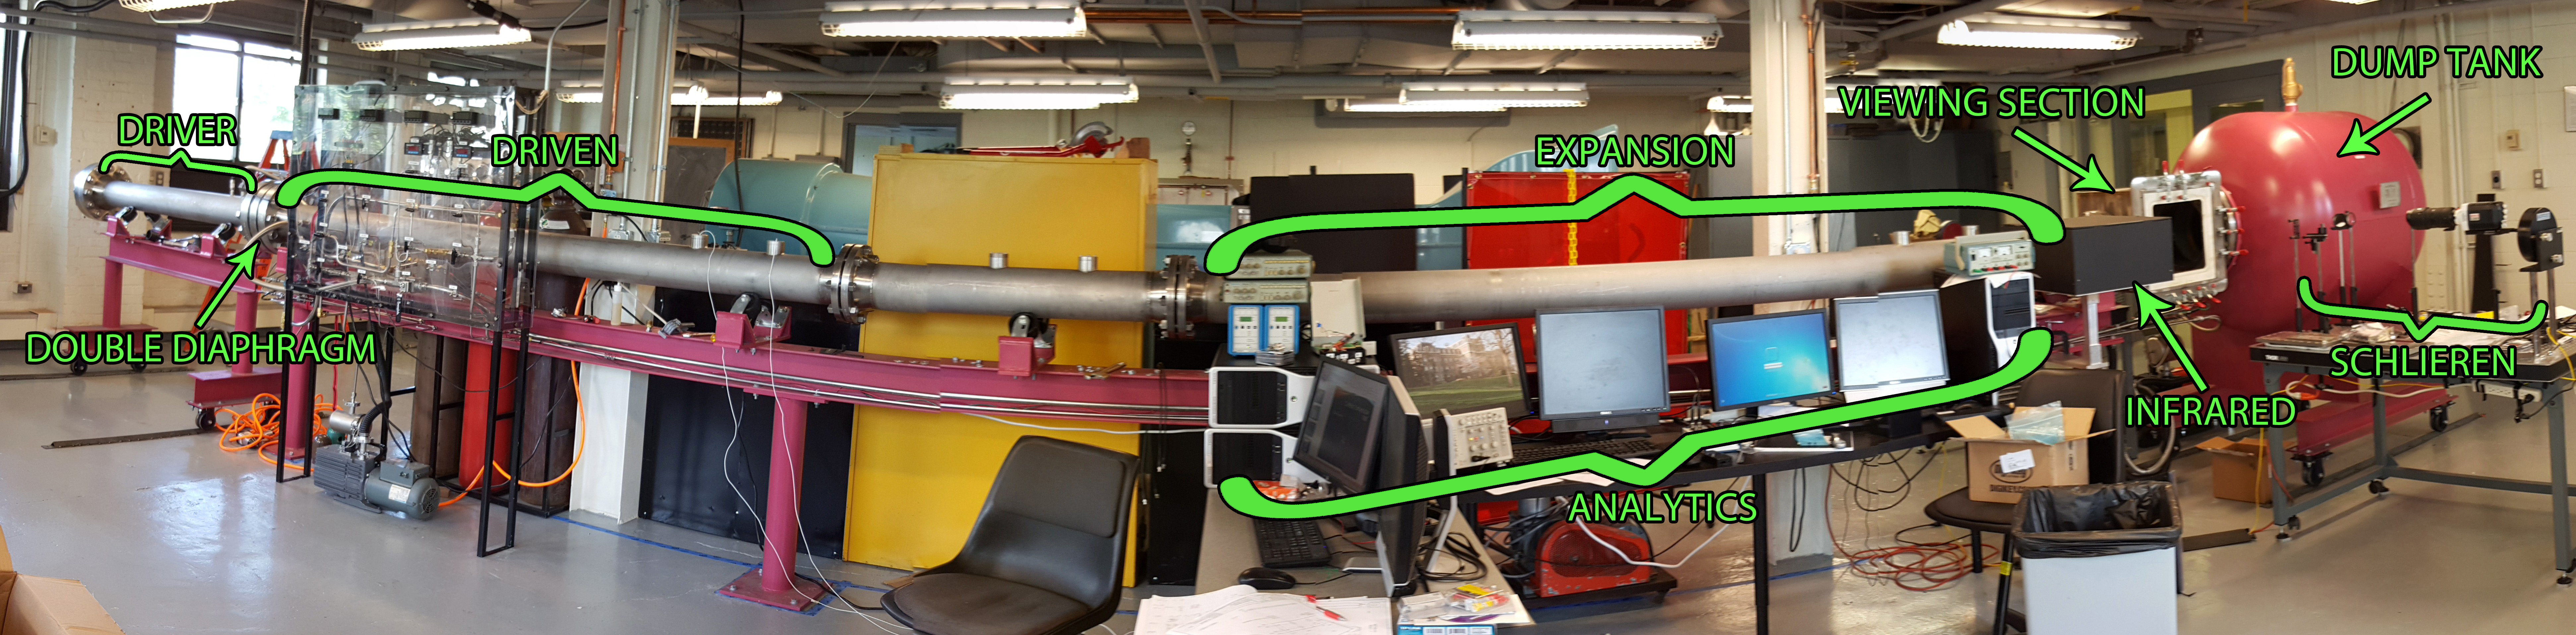
\includegraphics[width=\textwidth]{Figures/TubeLabeled.jpg}
\caption[Annotated Expansion Tube]{Annotated photograph of the expansion tube at Lafayette College}
\label{fig:tubelabeled}
\end{sidewaysfigure}

\begin{figure}
\centering
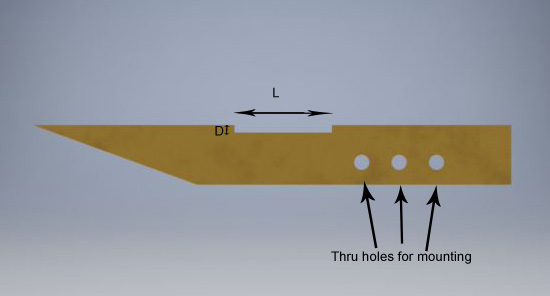
\includegraphics[height = 3in]{Figures/Cavitylabel.jpg}
\caption[Cavity 3D Model]{3D rendering of cavity used in testing}
\label{fig:cavModel}
\end{figure}

\begin{figure}
\centering
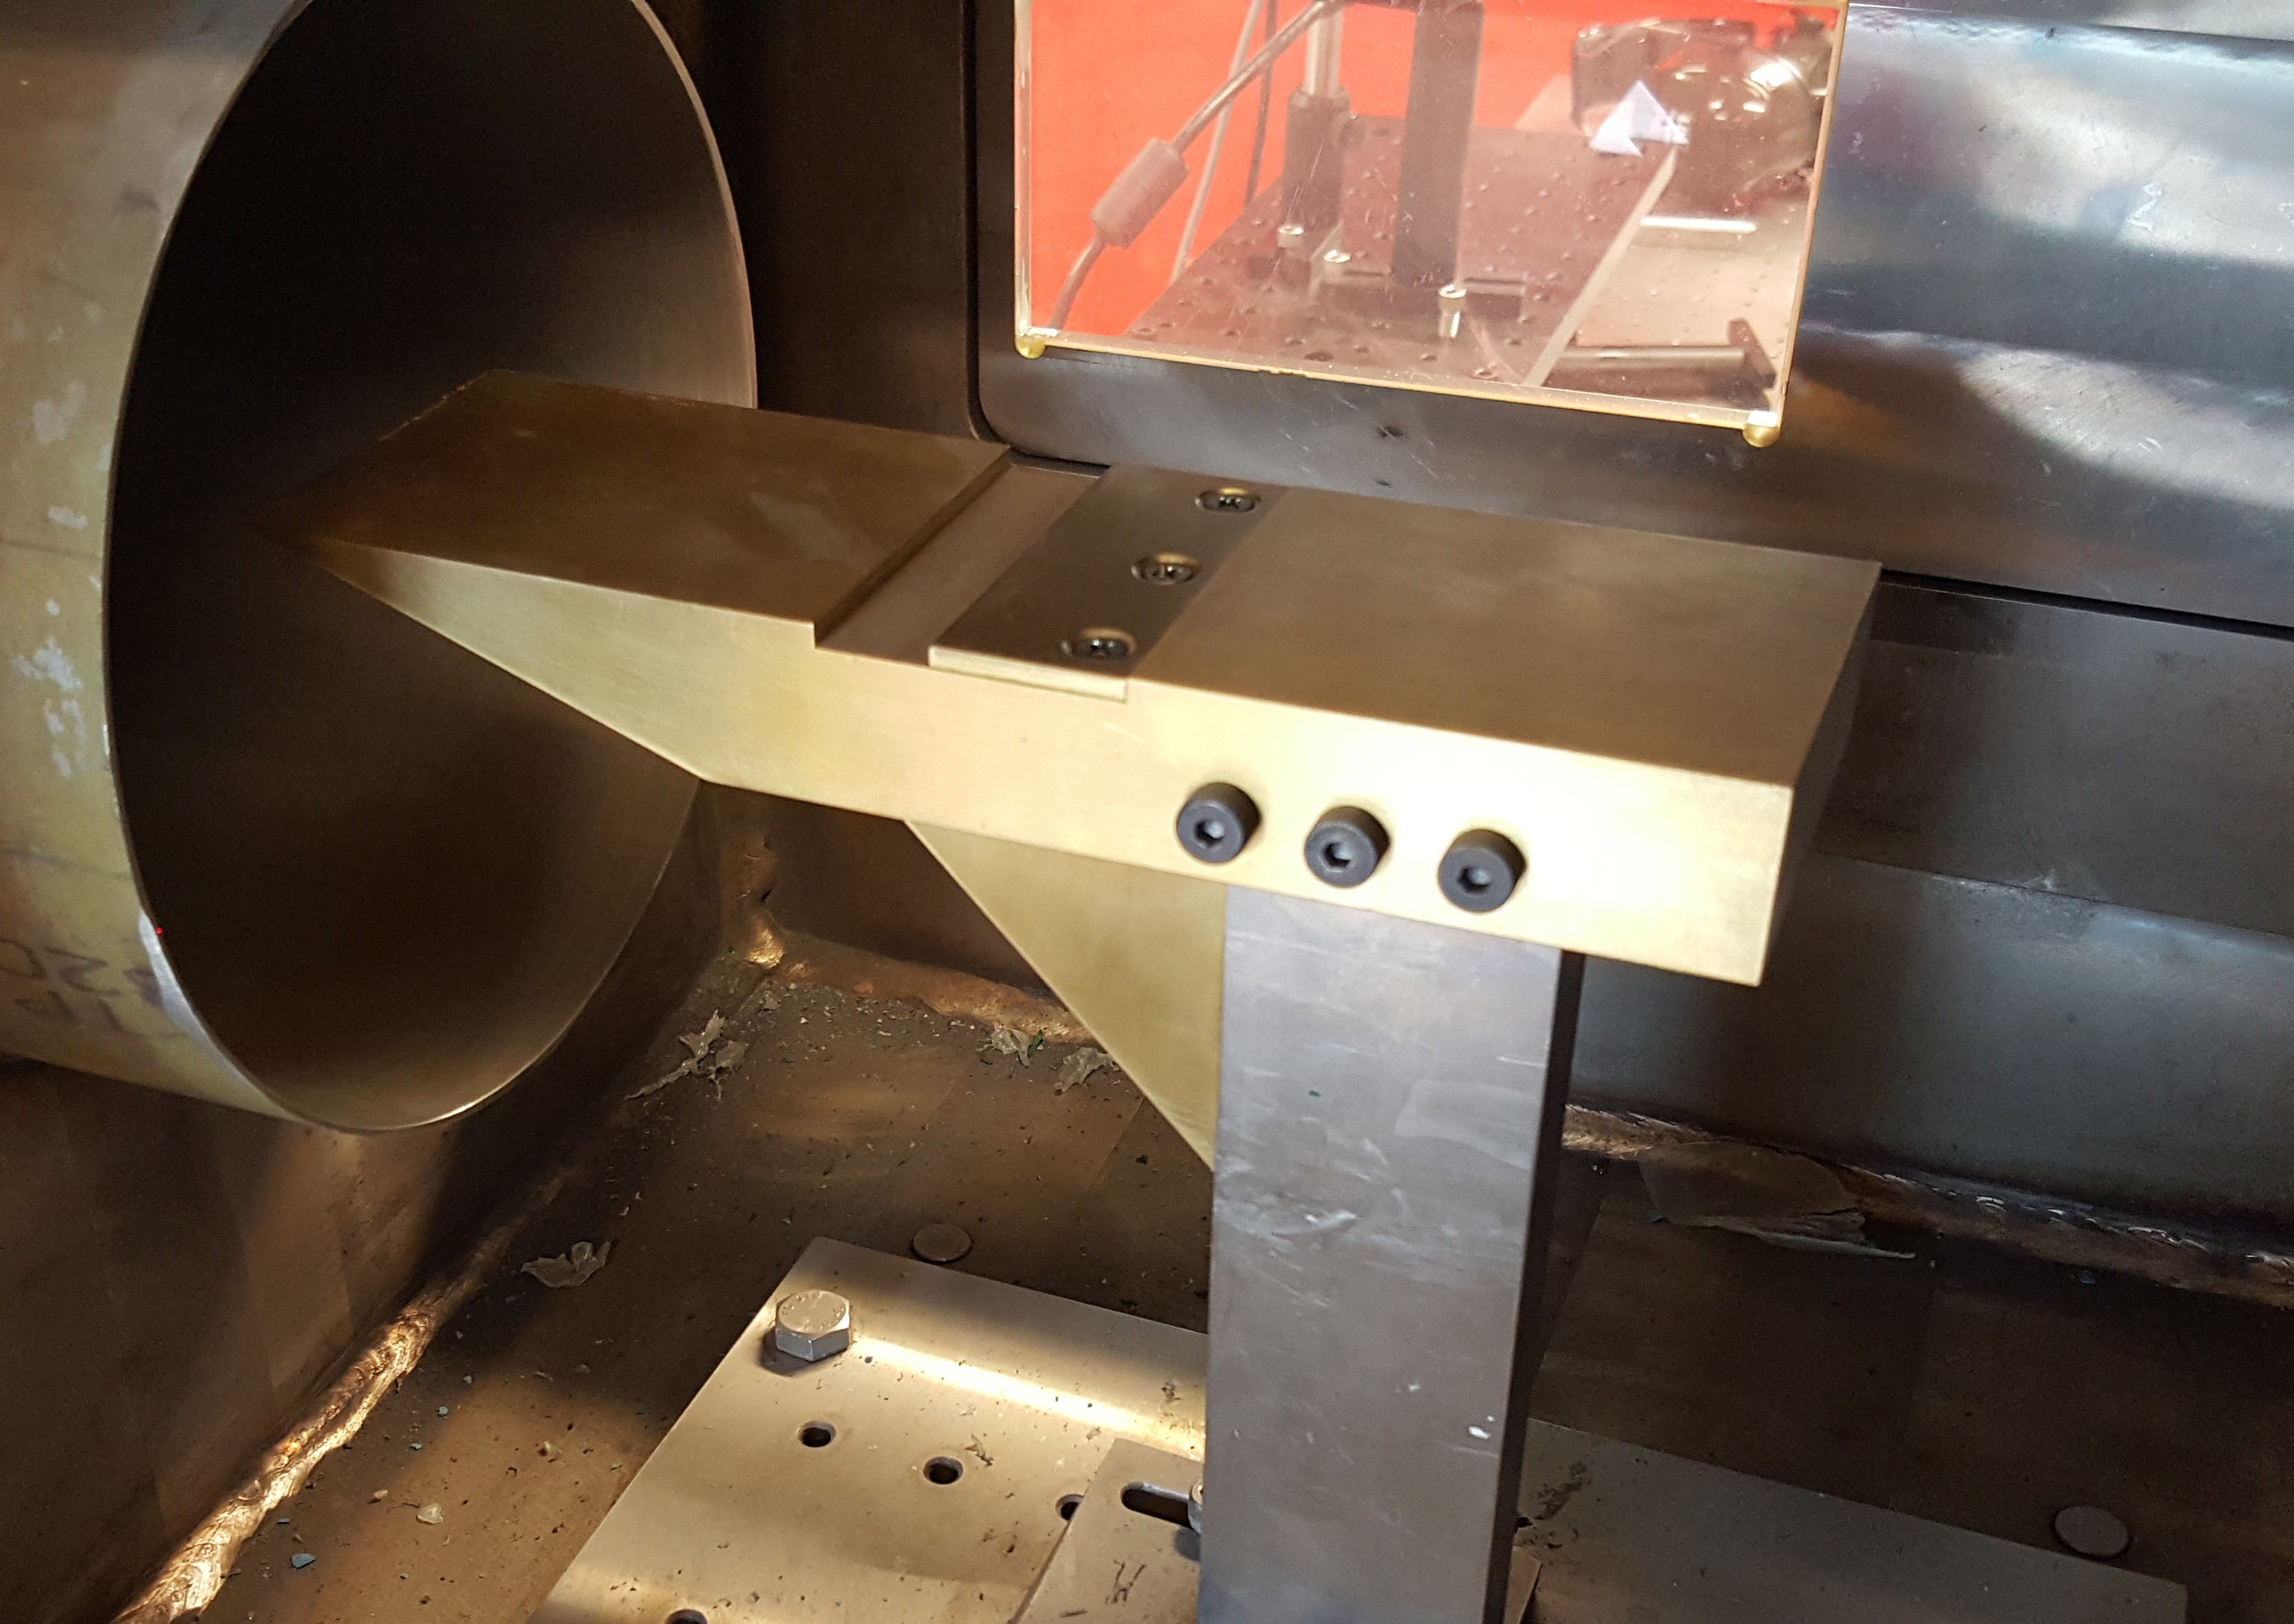
\includegraphics[height = 3in]{Figures/cavPhoto.jpg}
\caption[Cavity in Test Section]{Picture of cavity mounted in the test section.}
\label{fig:cavTestSection}
\end{figure}

\begin{figure}
\centering
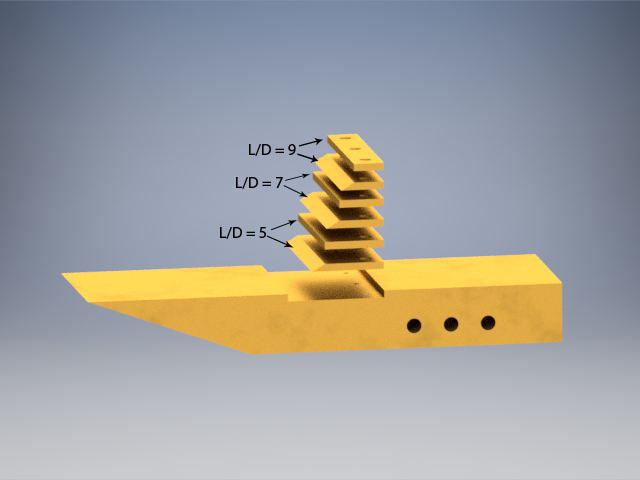
\includegraphics[height = 3in]{Figures/CavityInserts.jpg}
\caption[Cavity Model with Inserts]{3D rendering of cavity with various inserts to alter L/D}
\label{fig:cavInserts}
\end{figure}

\begin{figure}
\centering
\includegraphics[width=\textwidth]{Figures/Circuit.png}
\caption[Circuit Diagram for Timer Counter Box]{Circuit diagram for timer counter box}
\label{fig:timercircuit}
\end{figure}


\begin{figure}[p!]
\centering
\includegraphics[width=\textwidth]{Figures/DataFlow.png}
\caption[Data Flow for High Speed Pressure Transducers]{Data flow for high speed pressure transducers}
\label{fig:DataFlow}
\end{figure}
\clearpage

\begin{figure}
\centering
\includegraphics[height = 3in]{Figures/IRschematic.png}
\caption[IR setup diagram]{Schematic of the IR setup for the expansion tube.}
\label{fig:IRschematic}
\end{figure}

\begin{figure}
\centering
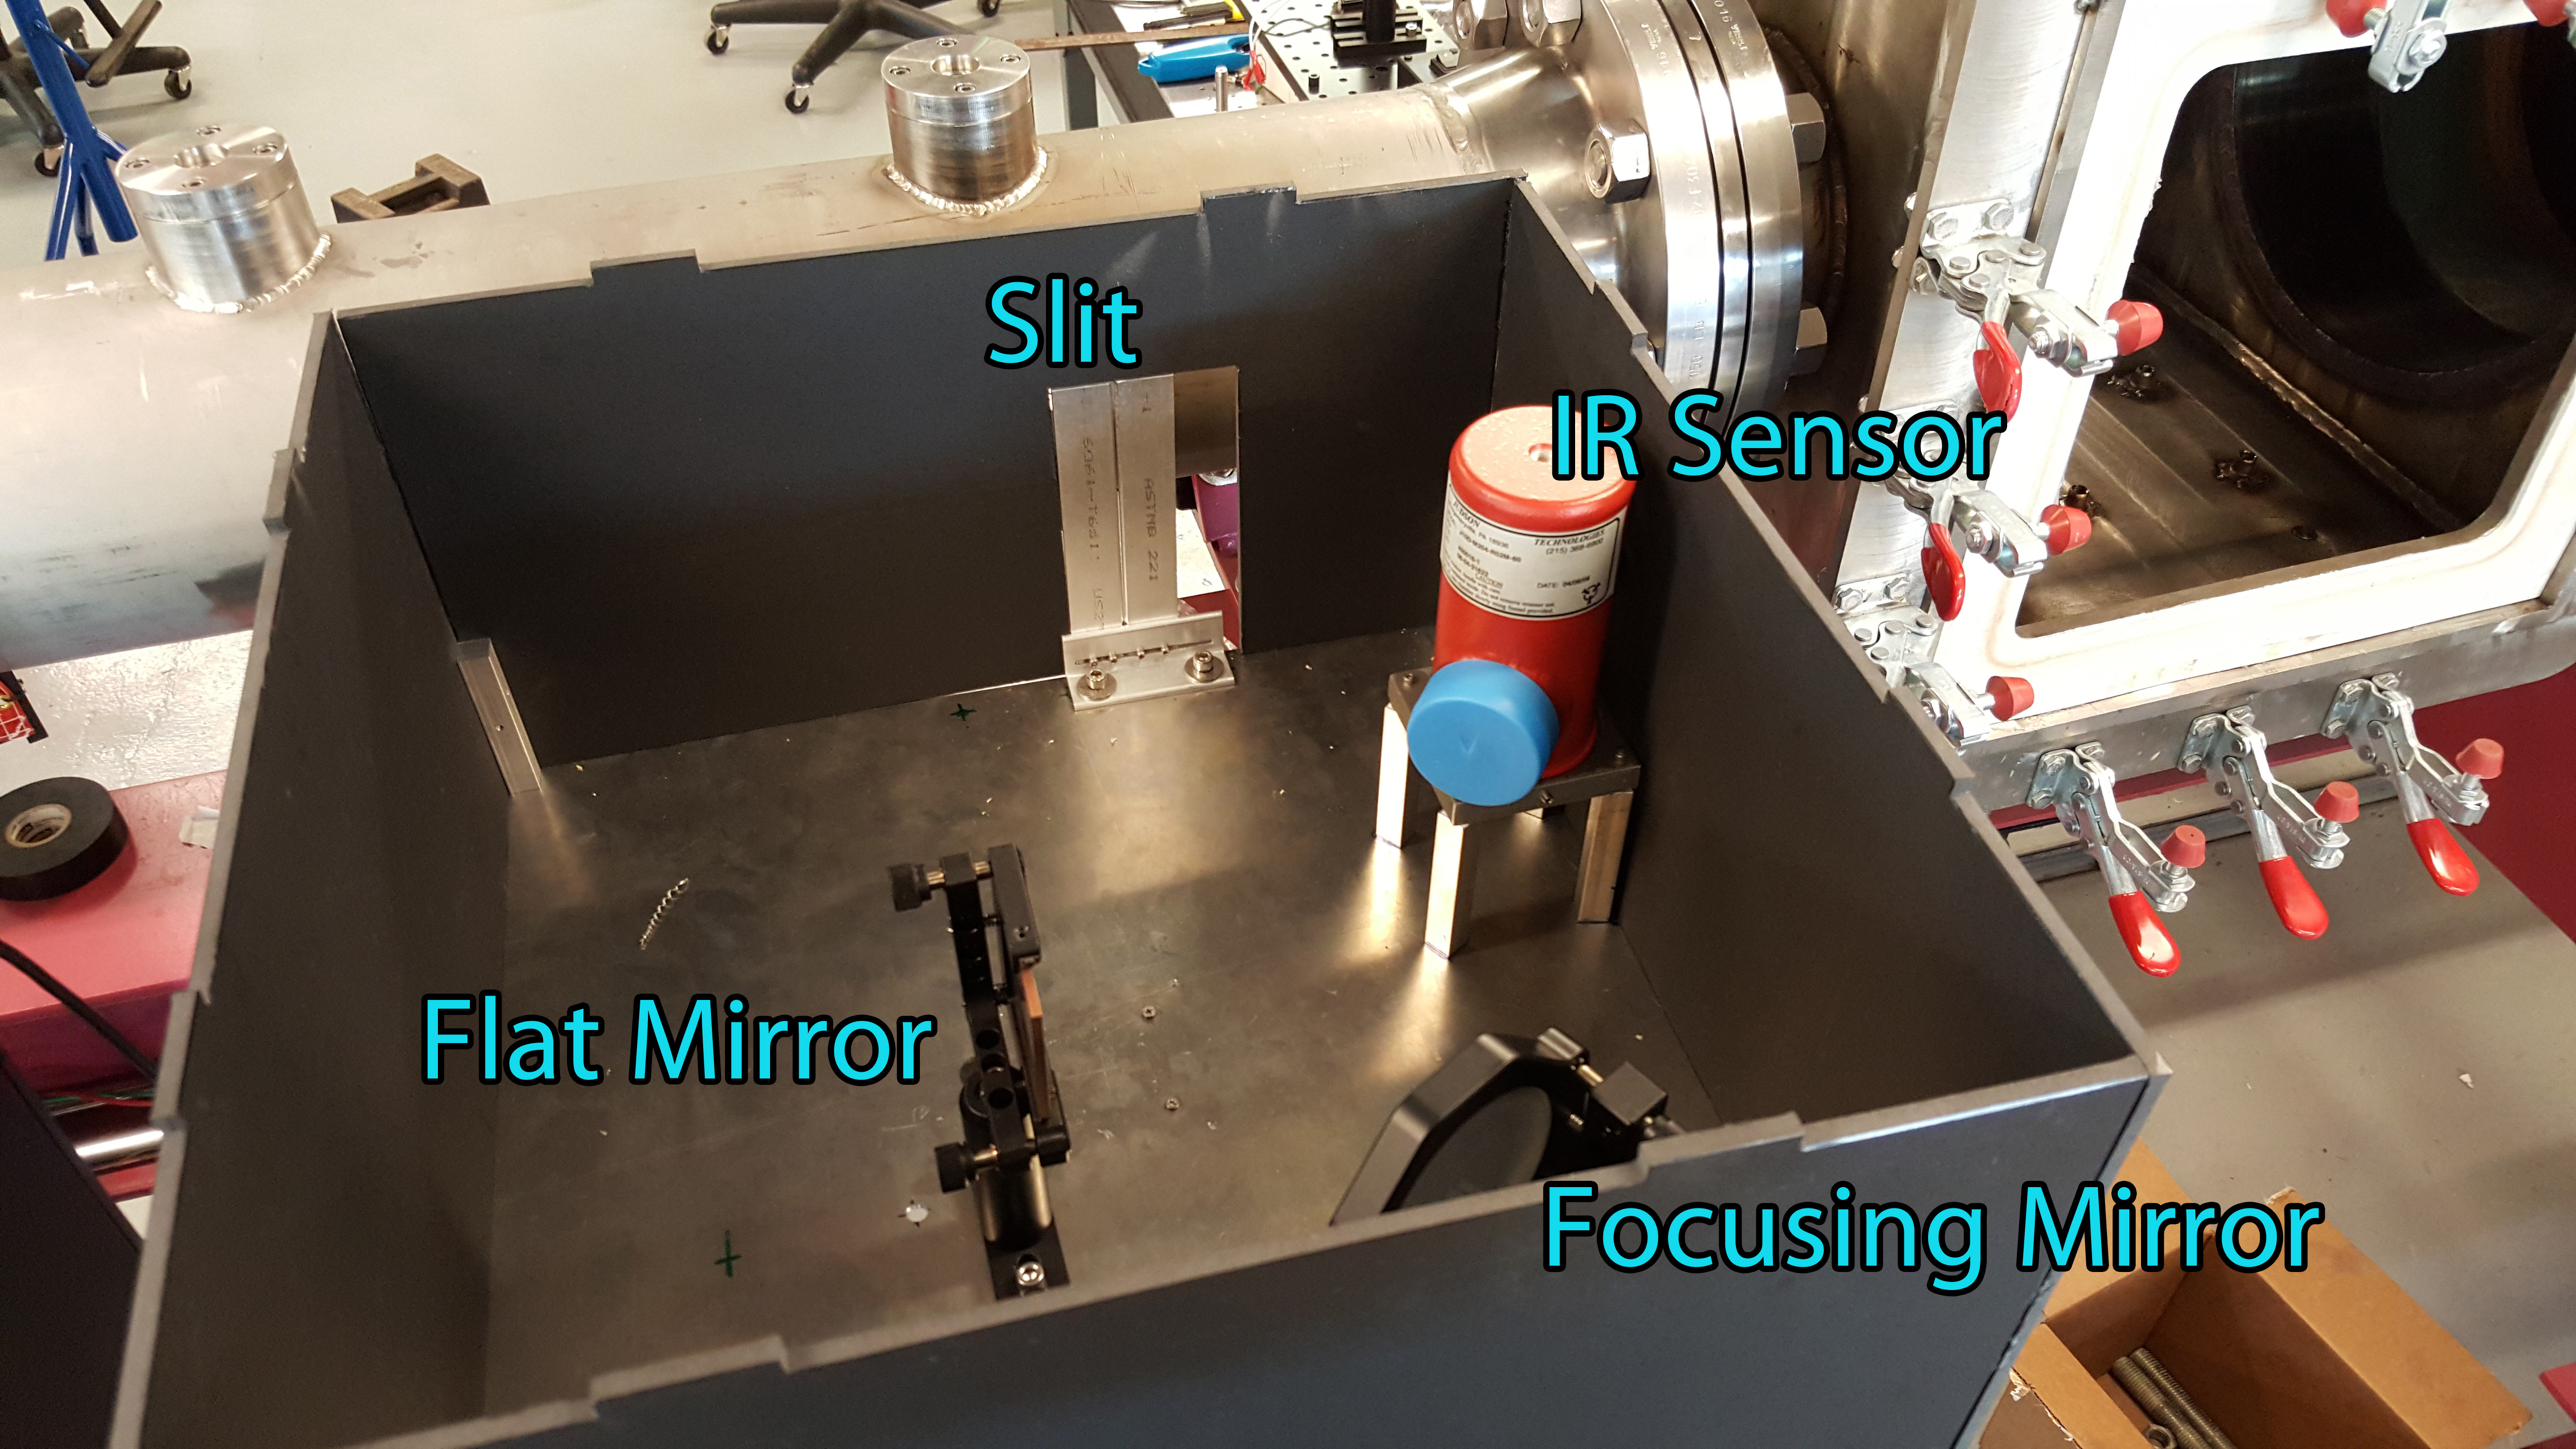
\includegraphics[height = 3in]{Figures/IRLabeled.jpg}
\caption[Labeled photograph of IR setup]{Photograph of actual IR setup in the lab.}
\label{fig:IRlabel}
\end{figure}

\begin{figure}
\centering
\includegraphics[height = 3in]{Figures/absorption.jpg}
\caption[Typical IR data utilizing absorption method]{Typical IR data utilizing absorption method}
\label{fig:IRabsorption}
\end{figure}

\begin{figure}
\centering
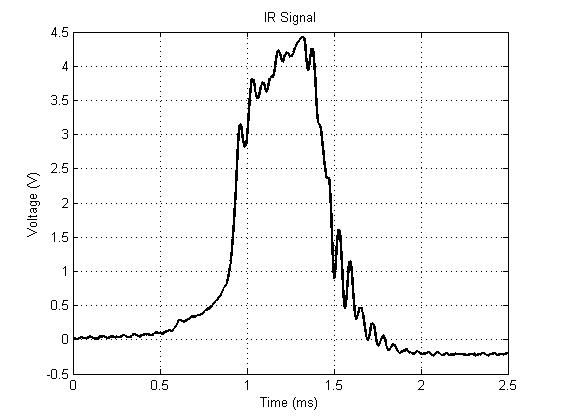
\includegraphics[height = 3in]{Figures/Co2NoPressure.jpg}
\caption[Typical IR data utilizing emission method]{Typical IR data utilizing emission method}
\label{fig:IRemission}
\end{figure}

\begin{figure}
\centering
\includegraphics[width=\textwidth]{Figures/Schlieren.png}
\caption[Schlieren Diagram]{Diagram of schlieren system at Lafayette}
\label{fig:schlieren}
\end{figure}